\subsection{Analisi Within Country e Test dei
Segni}\label{sec:results_within_country}

%L'analisi Within Country ha mostrato come, per i Paesi che hanno ospitato le
%Olimpiadi nelle edizioni dal 1964 al 2024, ospitare l'evento abbia portato in
%tutti i casi tranne uno (USA 1996) un numero maggiore di medaglie rispetto alla
%loro performance media.

L'analisi Within Country dal 1964 al 2024 ha mostrato come ospitare abbia in
tutti i casi portato significativamente più medaglie (in percentuale, tra +0.9 e
+3.4, o +50.2\% e +373.4\%), tranne che per USA (-1.3, o -9.9\%) e Canada (solo
+0.1, o +3.7\%).


% il testo basta a descrivere i dati, non consumerei due slot tabella per questo
% e spearman. L'ho messo in result.

% comunque, unire la germania con quella ovest non è tanto corretto, come ho
% scritto da altre parti (sono confini diversi, Paesi diversi...)


% info generale da conclusione

%Tuttavia, analizzando l'andamento del medagliere per alcuni di questi Paesi, si
%può notare come nelle edizioni precedenti rispetto a quella ospitata ci sia
%stato un incremento graduale.


% informazioni generali, le diremo insieme per tutti

%Il picco avuto nell'edizione ospitata potrebbe avere una spiegazione nei
%maggiori investimenti nello sport fatti negli anni precedenti, anche in vista
%della notizia dell'accettazione da parte del comitato Olimpico della
%candidatura da parte di quello specifico Paese. Infatti, ai Paesi viene
%comunicato che saranno loro ad ospitare le Olimpiadi per una specifica edizione
%ben 7 anni prima, dando allo Stato tempo per iniziare ad investire nelle
%infrastrutture sportive.


% sposto l'interpretazione qui, così, stando vicino, si capiscono i risultati

%Il Test dei Segni ha confermato quanto può essere visionato anche ad occhi: il
%test ha calcolato infatti un p-value di 0.0034

Il \textbf{Test dei Segni} conferma il risultato: il \textbf{$p$-value di
0.0034} (sintomo di sbilanciamento tra i segni) permette di rigettare con
estrema confidenza l'ipotesi nulla $H_0$ e confermare l'esistenza di un
vantaggio sistematico nell'ospitare.

\cref{fig:host_performance_img} mostra spesso un picco in casa, ma suggerisce
anche una crescita iniziata prima.

\begin{figure}[H]
    \centering
    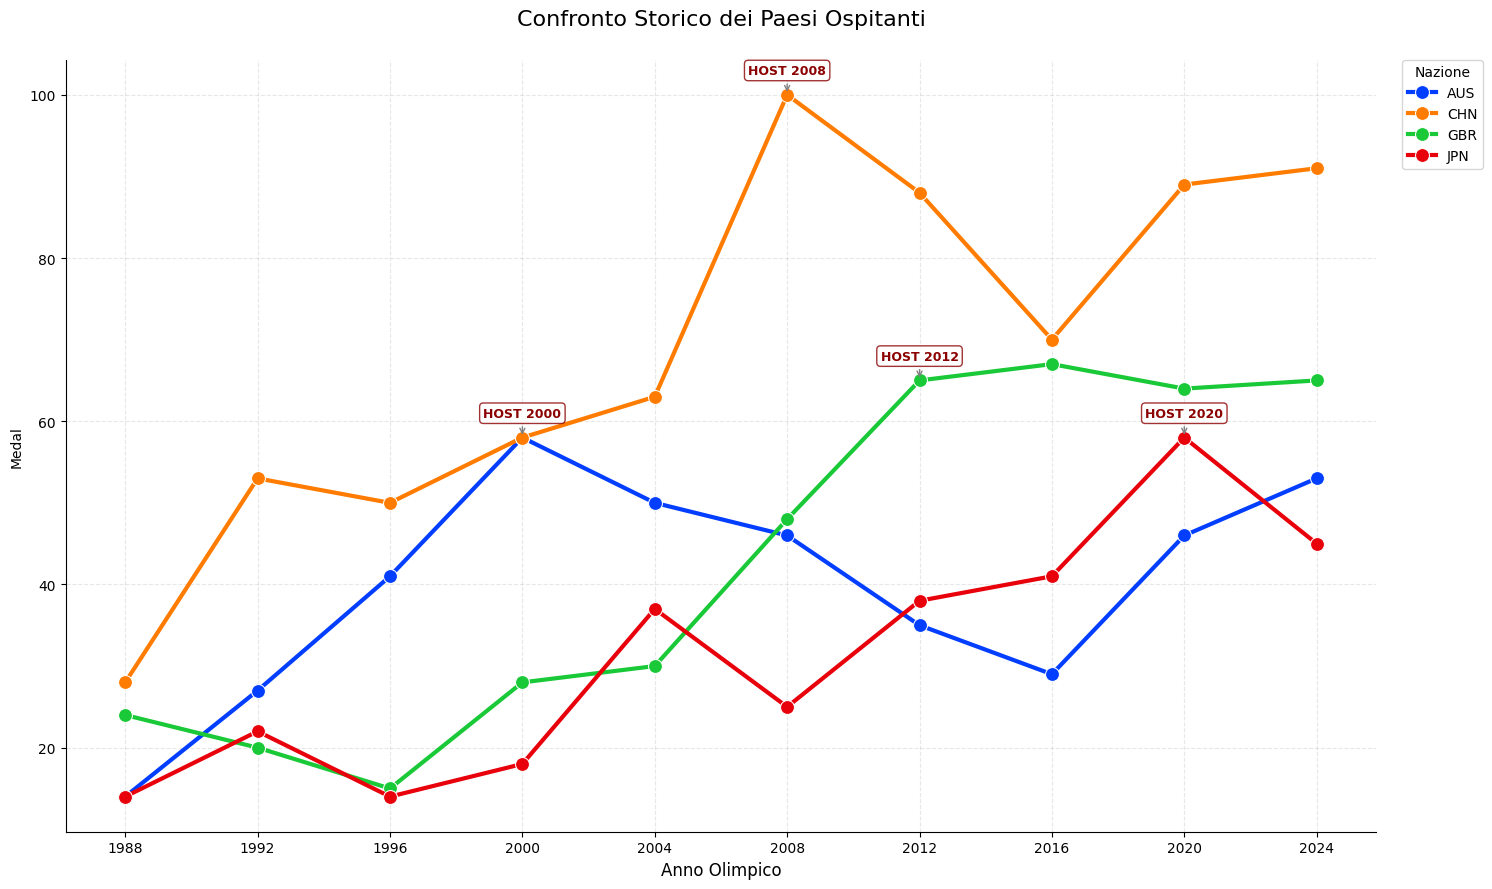
\includegraphics[width=\linewidth]{../../docs/img/Host_Performance.png}
    \caption{Performance 1988--2024 per alcuni Pesi host}
    \label{fig:host_performance_img}
\end{figure}